\UseRawInputEncoding
\documentclass[12pt, letterpaper] {article}
\usepackage{natbib}
\usepackage{amsmath, amsthm, amssymb, mathrsfs,array}
\usepackage{graphicx,float,wrapfig,subfigure,color,pdfpages,fixltx2e,url}


\pagestyle{plain}
\setlength{\parskip} {11pt}
\setlength{\parindent} {2em}
\setlength{\textwidth}{6.5in}
\setlength{\oddsidemargin} {0in}
\setlength{\textheight} {8.5in}
\setlength{\topmargin} {-0.5in}
\parskip 7.2pt

\newcommand{\nnub}{\nonumber}
\newtheorem{theorem}{Theorem}
\newtheorem{lemma}{Lemma}
\newtheorem{transform}{Transformation}
\newtheorem{corollary}{Corollary}
\newtheorem{property}{Property}
%\newtheorem{proposition}{Proposition}[section]
\newtheorem{proposition}{Proposition}
\newtheorem{definition}{Definition}
\newtheorem{algorithm}{Algorithm}
\newtheorem{assumption}{Assumption}
\newtheorem{observation}{Observation}

\renewcommand{\baselinestretch}{1.5}

\newcommand{\vocab}[1]{\textcolor{red}{#1}}

\begin{document}
	\title{NUS Business School Honors Dissertation}
	\author{Peng Seng Ang}
	\date{AY 2019/2020 Semester 2}
	\maketitle
\begin{abstract}
\noindent Many real industry problems involves spatio-temporal demand prediction (e.g predicting demand at a certain time across different locations). Most of the demand data are not continuous variables but instead count variables, like number of orders and number of transactions. This paper studies how we can apply time series model to count variables, using VAR models to exploit spatial correlations as well as introduce a 3-step approach to improve forecast accuracy. 

\end{abstract}
\section{Introduction}

The motivation for this paper comes from \cite{Sheng2018}, where their focus is to optimise assignments of orders to drivers in order to minimize the total delay of all drivers. The dataset used in both \cite{Sheng2018} and this paper are from a food service provider in China that allows customer to place orders before a cutoff time in the day (e.g 10.00am) and the customer can expect to recieve their orders by a deadline (e.g anytime from 10.30am to 11.45am). 

\noindent The problem is not only restricted to the abovementioned food provider. With the rise of e-commerce and the food ordering and delivery services, like GrabFood and FoodPanda, demand prediction and driver assignment problem would be an everyday concern for them too. 

\noindent In reality, demand is never deterministic and hence, having an accurate forecast of demand for the food service providers would help them more effectively and efficiently assign orders to drivers to improve the overall delivery time. As such, the focus of this paper would be to accurately model and forecast the demand at the different locations and time. Currently, most Autoregressive (AR) or Autoregressive Integrated Moving Average (ARIMA) models only consider temporal features when predicting demand. However, we believe including spatial features between the data points might improve forecast accuracy. This paper would focus on and explore models that include both spatial and temporal features to improve forecast accuracy. 

\section{Literature Review}
\cite{Marina2016} describes and shows how they implemented a network autoregressive moving average model to model the number of cases of Mumps in UK counties. In their example, they also showed that they might achieve a better result by modelling the series separately as univariate time series, also suggested in \cite{Nunes2015} since the neighbouring counties does not provide a substantial amount of explanatory power.  Other related literature includes \cite{Xavier2005} where they propose a model building strategy for spatially sparse but temporally rich data. 

\noindent BigVAR and tscount are some libraries that would be used in this paper. \cite{Tobias2017} provides the mathematical background and implementation of Generalised Linear Models (GLM) for count time series as a library (tscount) in R while \cite{William2017} extensively descibes the background and implementation of the VAR models and BigVAR library for multi-variate time series.

\noindent There are also various research on different methods used to predict spatio-temporal demand. One example would be \cite{Abolfazl2017}, where they proposed using generalized spatio-temporal autoregressive model for predicting taxi demands across locations in New York City. 

\section{Data}
The data source used was an operational dataset from a food delivery service provider from Shanghai that includes delivery information for a 2-month period from 10 August 2015 to 30 September 2015 (excluding Saturdays) in 2015. The provider only provides delivery service for 90 minutes during lunchtime and the dataset has split the data into 15-minute time periods, and as such, each day would only consists of demand data for 6 time periods. Hence, our dataset has 839 locations with demand count data, in integer, for 204 time periods in total. 

\noindent To include other exogenous variables, data from https://www.worldweatheronline.com/shanghai-weather-history/shanghai/cn.aspx was used to include weather and rainfall data as well as encoding of the weekadys for all the respective days. 

\subsection{Exploratory Analysis}
We would first do some exploratory analysis and check if there are any interesting relationships between the variables. 

\begin{figure}[H]
    \centering
    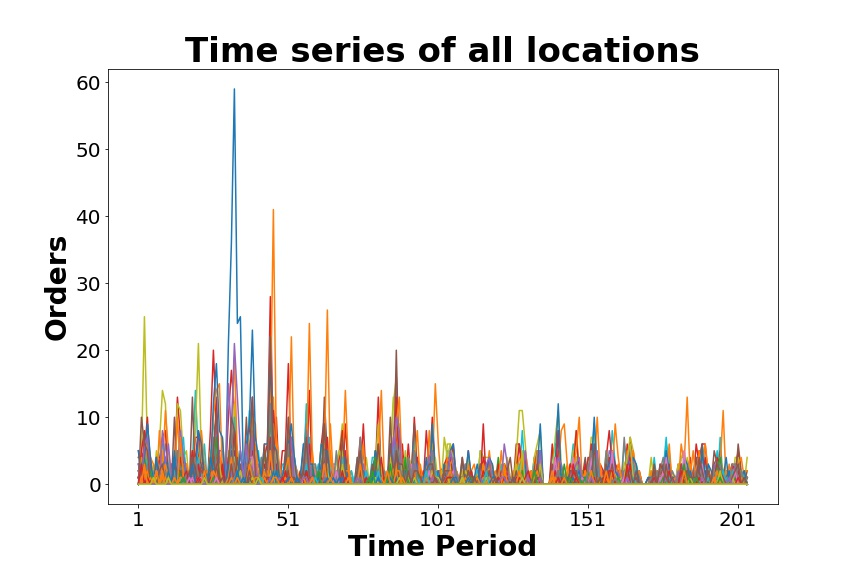
\includegraphics[width=0.95\textwidth, height=0.7\textheight]{Images/example_all_ts.jpg}
    \caption{Time series of all locations in the dataset. It can be observed that most locations have very low number of orders across the time period.}
    \label{fig:Time series of all locations in the dataset. It can be observed that most locations have very low number of orders across the time period.}
\end{figure}


\begin{figure}[H]
    \centering
    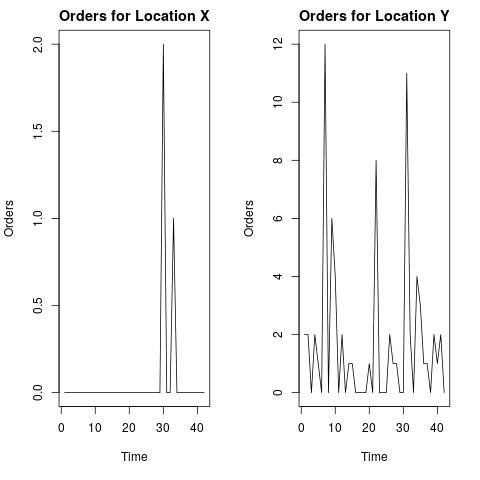
\includegraphics[width=\textwidth, height=0.4\textheight] {Images/example_ts.jpg}
    \caption{Most locations have very sparse time series (left) while some have relatively more dense time series (right)}
    \label{fig:Most locations have very sparse time series (left) while some have relatively more dense time series (right)}
\end{figure}


\begin{figure}[H]
    \centering
    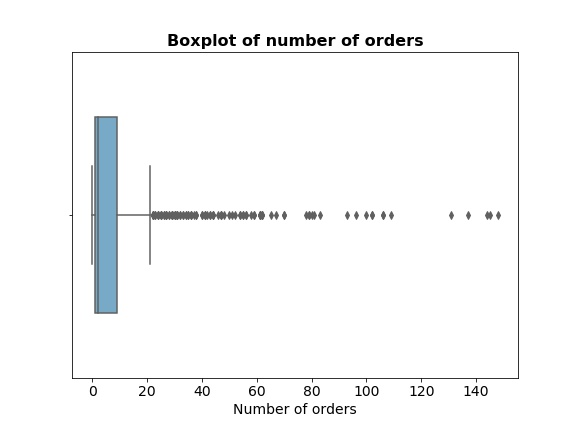
\includegraphics[width=0.95\textwidth, height=0.4\textheight]{Images/boxplot_counts.jpg}
    \caption{Boxplot of counts}
    \label{fig:Boxplot of counts}
\end{figure}

\noindent We can see from the boxplot in Figure 3 that most of the locations have extremely low number of non-zero orders and further analysis showed that about 335 locations have just a maximum of one non-zero order throughout the 204 time periods. 

\noindent Analysis on some exogenous factors were performed too. 
\begin{figure}[H]
    \centering
    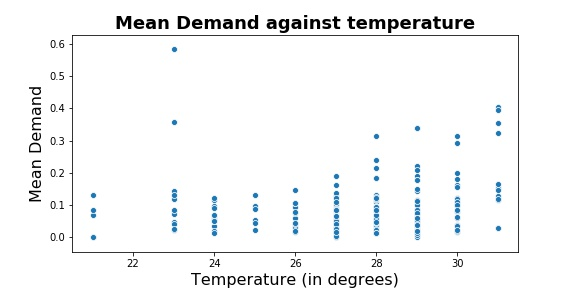
\includegraphics[width=0.95\textwidth, height=0.32\textheight]{Images/temp_mean_demand.jpg}
    \caption{Scatter plot of mean counts against temperature}
    \label{fig:Scatter plot of mean counts against temperature}
\end{figure}

\begin{figure}[H]
    \centering
    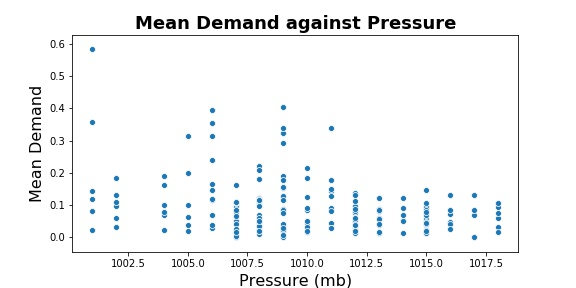
\includegraphics[width=0.95\textwidth, height=0.32\textheight]{Images/pressure_mean_demand.jpg}
    \caption{Scatter plot of mean counts against pressure}
    \label{fig:Scatter plot of mean counts against pressure}
\end{figure}

\noindent The scatter plot in Figure 4 visually display a slight positive relationship between temperature and mean demand across all locations whereas Figure 5 visually display a slight negative relationship between pressure and mean demand across all locations.  


\subsection{Train-Test Split}
From Figure 1 in Section 3.1, the data is very sparse as there are many locations that have no demand counts for the majority of the time period. Hence, to get a better idea of how our models would work, only locations with at least 50 non-zero counts across the time period would be used initially, leaving us with 42 locations that meet this criteria. After the model is tested on the smaller dataset, we would then use the full dataset for location with at least one non-zero count to test and fit our model. 

\noindent The dataset was then split into training and test set by considering the first 33 days as the training set and the next 1 day as the test set. Our training set would then have 198 demand data for each location and test set would have 6 demand data for each location. 

\section{Baseline Model}
In this section, we would build a simple baseline model. Following which, we would try other different spatial temporal time series models and compare the results to the baseline model. 

\subsection{Metric Used}
The main metric that would be used for comparison would be Mean Squared Forecast Error (MSFE), which is calculated by:

\begin{center}
    %$\displaystyle MSFE=\frac{1}{(T_2 - T_1 - 1)}\sum_{t=T_1}^{T_2 - 1}\left \| \hat{y}_{t+1} - y_{t+1} \right \|_{2}^{2}$
    $\displaystyle MSFE=\frac{1}{n}\sum_{t=1}^{n}\left \| \hat{y}_{t} - y_{t} \right \|_{2}^{2}$
\end{center}
where \textit{n} is the number of data points, $\hat{y_t}$ is the predicted demand at time t and ${y_t}$ is the actual demand at time t.


\subsection{ARIMA models}
Autoregressive Integrated Moving Average (ARIMA) models are one of the most commonly used models for time series (\cite{Asha2016}). ARIMA models are made up of 3 processes, mainly the Autoregressive (AR) process, the Integrated (I) process and the Moving Average (MA) process (\cite{Jamal2018}). The AR process assumes that each observation can be expressed as a linear combination of its past values.  An AR(x) process would mean using x lagged values. The MA process assumes that each observation can be expressed as a linear combination of its current error term as well as its past error terms. The Integrated Process states that the time series can undergo differencing to ensure that the series is stationary. A MA(x) process would mean using x number of past observations. Hence, an ARIMA model is usually represented by ARIMA(p,d,q), where \textit{p} represents the number of autoregressive terms, \textit{d} represents the number of differences needed for stationarity, and \textit{q} represents the number of lagged forecast errors. 

\subsection{Baseline ARIMA Result}
As a baseline model, each of the locations was assessed individually and a suitable ARIMA model was built for each location. Auto-arima function from Python was used to implement this. The out-of-sample MSFE for this baseline model on the 42 locations is \textbf{73.29}. A sample forecast plot is shown below:

\begin{figure}[H]
    \centering
    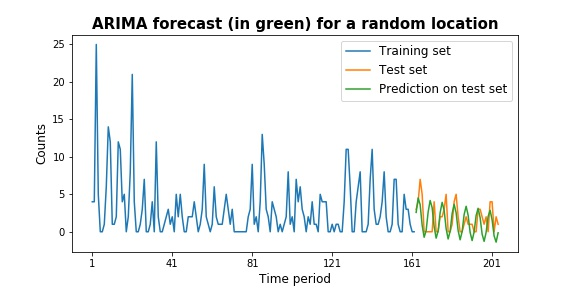
\includegraphics[width=\textwidth]{Images/forecast_example.jpg}
    \caption{ARIMA forecast on a random location}
    \label{fig:ARIMA forecast on a random location}
\end{figure}


\section{GLM Model}
The dataset that we are using follows a count time series, which means the observations are non-negative integers. A flexible and commonly used model for count time series is the Generalized Linear Model (GLM) \cite{Nelder1972}. GLM normally take the form of:

\begin{center}
    $\displaystyle g(\lambda_t)= \eta^T X_t$
\end{center}

\noindent Using the R package from \cite{Tobias2017}, the GLM used would be an extension of the above equation and can be expressed in the form of:

\begin{center}
    $\displaystyle g(\lambda_t)=\beta_0 + \sum_{k=1}^{p}\beta_k\tilde{g}(Y_{t-i_k}) + \sum_{\mathit{l}=1}^{q}\alpha_\mathit{l} g(\lambda_{t-j_\mathit{l}}) + \eta^T X_t$
\end{center}

\noindent where $g$ represents a link function and $ \tilde{g}$ represents a transformation function. $\eta$ represents a parameter vector that corresponds to the covariates. 

\subsection{Model Implementation}
\noindent Since there are many locations which have values that are all 0 throughout all the time period, the GLM model would run into an error if applied on those. Hence, only locations with at least 1 non-zero value would be considered. Similar to before, each of the locations was assessed individually and a suitable GLM model was fitted for each location. The out-of-sample MSFE for this baseline model is \textbf{82.42}. 

\subsection{Model Diagnostics}
To validate and verify if our fitted model is adequate, model checking would be performed by performing the following residual analysis.	

\subsubsection{Residuals plots}

\begin{figure}[H]
    \centering
    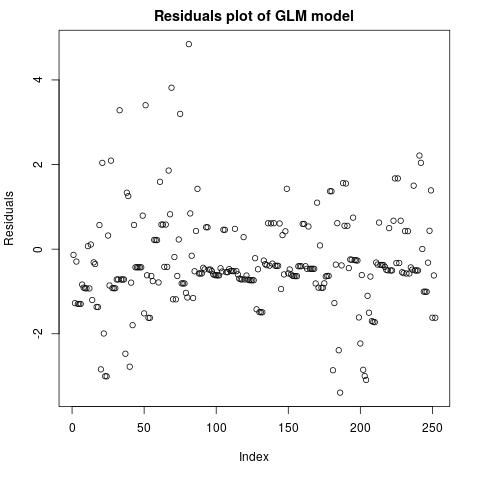
\includegraphics[width=\textwidth, height=0.4\textheight]{Images/Full_GLM_resids.jpg}
    \caption{Residuals for GLM Model}
    \label{fig:Residuals for GLM Model}
\end{figure}

\noindent Figure 7 diagnostic plots shows that while the residuals roughly randomly scattered, the GLM model produces residuals that does not follow the normal distribution well. This is expected as we assume that the distribution is poisson and not normal. 

\subsubsection{Residuals against Predicted values}

\begin{figure}[H]
    \centering
    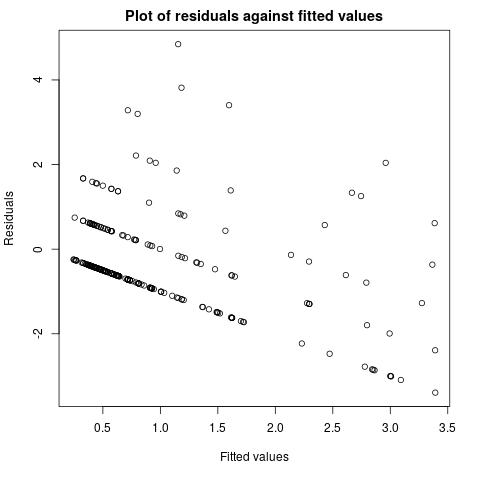
\includegraphics[width=0.85\textwidth, height=0.6\textheight]{Images/Full_GLM_resids_vs_fitted.jpg}
    \caption{Residuals against Predicted values for GLM Model}
    \label{fig:Residuals against Predicted values for GLM Model}
\end{figure}

\noindent The above plot of residuals against the predicted values suggests heteroscedasticity between residuals, or non-constant variance between the residuals as the predicted value increases, which is expected in a Poisson GLM, as mentioned in \cite{Dylan2017}. For a normal regression model, this is a bad sign but since we are assuming that our count data follows a Poisson distribution, the residuals are bound to display heteroscadasticity. 

\subsection{Model Limitation}

The MSFE of the GLM model is better than that of the baseline model. However, it would be relatively expensive and time-consuming as every location has to be individually fitted to a GLM model. Also, it only uses its past values and does not take into account data from the other locations. The next section explores another type of model which would use data from other locations. 

\section{VAR Model}

\subsection{Motivation}

As with many spatio-temporal demand prediction, spatial features could be an important feature if there exist spatial correlation. To check if there exist spatial correlation between the locations, a correlation heatmap would be plotted. For clear illustration purposes, instead of showing the matrix of correlation for all 839 locations, only the 42 locations with at least 50 non-zero counts would be shown. 

\begin{figure}[H]
    \centering
    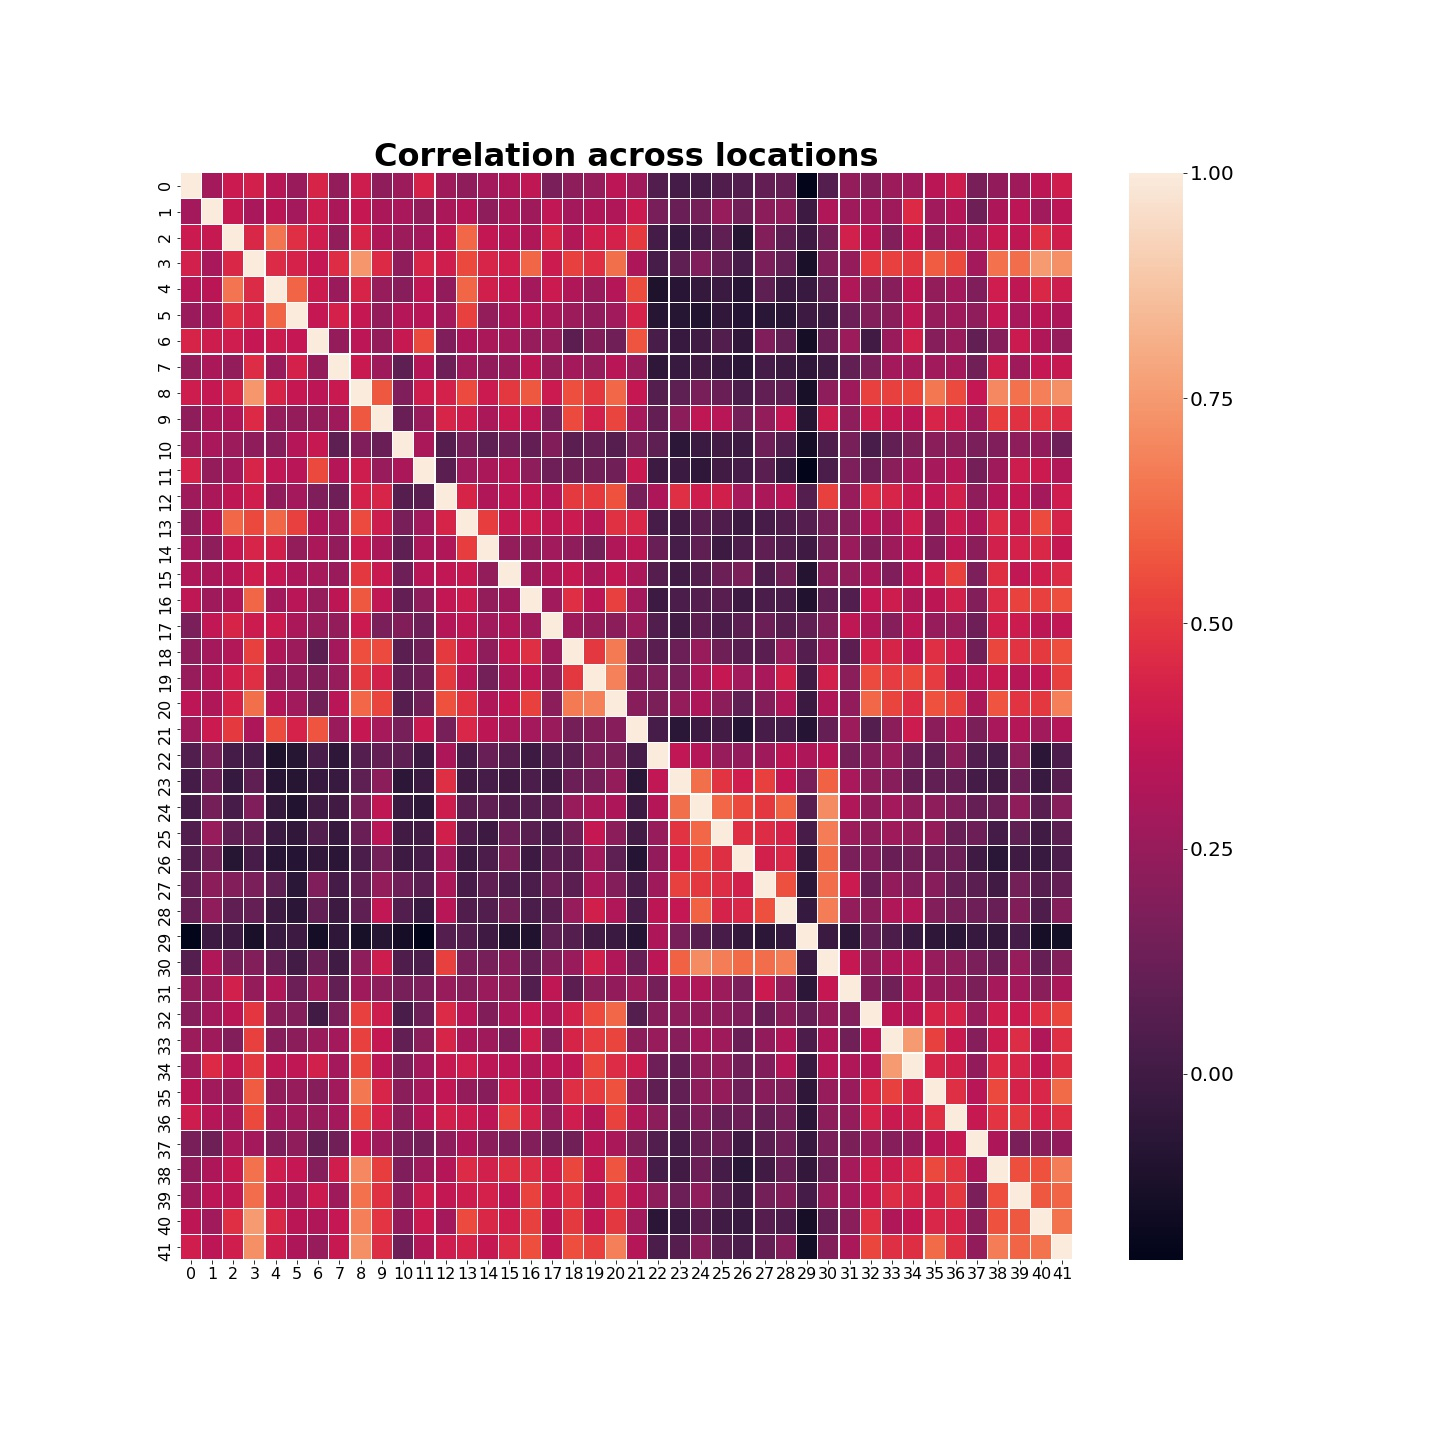
\includegraphics[width=\textwidth, height=0.9\textheight]{Images/heatmap.jpg}
    \caption{Spatial Correlation Heatmap on the locations with at least 50 non-zero counts. Axes represent the 42 locations}
    \label{fig:Spatial Correlation Heatmap. Axes represent locations}
\end{figure}

This provides the motivation to use the existence of spatial correlation and explore the usage of VAR model.


\subsection{Details of VAR Model}
Vector Autoregressive (VAR) models are the most commonly used model for multivariate time series, particularly in economics and financial time series as shown in \cite{Hilde2000}. VAR models are very similar to multivariate linear regression models and methods used to perform inferencing on linear regression models can also be applied to VAR models. VAR(p) represents a VAR model of order p if the time series can be written as: 

\begin{center}
    $\displaystyle y_t=v+\sum_{i=1}^{p} \phi_{i}y_{t-i}+\alpha_t$
\end{center}

\noindent where $p$ is the number of lagged endogenous variables used, $y_t$ is the value at time $t$, $v$ is a constant vector, $\phi_i$ are coefficient matrices for $i>0$ and $\alpha_t$ are independent and identically distributed random vectors. 

\subsection{Stationarity Condition}
For a univariate time series, it is important for the time series to be transformed into a stationary series and Augmented Dickey-Fuller (ADF) test can be used to perform unit root test for stationarity, as shown in \cite{Zhijie1998} and \cite{Rizwan2011}. For a multi-variate time series, if the series are unit-root non-stationary, applying the VAR model could lead to spurious regression, as shown in \cite{Baumohl2009}.  

\subsubsection{Cointegration}
\cite{Box1977} shows that it is possible to linearly combine various unit-root nonstationary time series to form a stationary series. The term Cointegration, first mentioned in \cite{Granger1983}, states that although some or all the time series might be unit-root nonstationary individually, these time series can be said to be cointegrated if there exists a possible linear combination of them that would form a stationary series. Intuitively, 2 series are cointegrated if they move together and the distance between them remain stable over time. 

\subsubsection{Johansen Test for Cointegration}
While Cointegrated Augmented Dickey Fuller Test, commonly used for Pairs Trading, can be used, it is only able to be applied on 2 separate series. In our dataset, we have 839 locations at least, hence we would apply the popular approach to cointegrating tests for VAR model, called the Johansen's Cointegration Test. However, one limitation is that it can only be used to check for cointegration between a maximum of 12 variables. For further elaboration on the Johansen's Cointegration Test, please refer to \cite{Johansen1991}. Since our dataset has 839 variables (locations), we are unable to accurately calculate the significant values of more than 12 variables and hence unable to determine correctly the number of cointegration vectors needed. 

\subsubsection{Differencing}
Instead, differencing would be performed on every series to make the series levels stationary. After differencing, ADF test was performed on each series and the following result shows that all the series are stationary. 

\noindent The time series of each location have been checked and are stationary. 
While it is possible to perform differencing on every series, it might cause over-differencing, as mentioned in \cite{Ruey2014}.

\subsection{VARX Model}
VAR models can also be extended to include exogenous variables. A VARX(p,s) (with exogenous variables) model can be expressed as:

\begin{center}
    $\displaystyle y_t=v+\sum_{i=1}^{p} \phi_{i}y_{t-i}+\sum_{j=1}^{s} \beta_{j}x_{t-j}+\alpha_t$
\end{center}

\noindent where $p$ is the number of lagged endogenous variables used, $s$ is the number of lagged exogenous variables used, $y_t$ is the value at time $t$, $v$ is a constant vector, $\phi_i$ are coefficient matrices for endogenous coefficient matrix for $i>0$, $\beta_i$ are coefficient matrices for exogenous coefficient matrix for $i>0$ and $\alpha_t$ are independent and identically distributed random vectors. 

\noindent Our dataset uses additional exogenous variables like temperature, wind, gust, cloud, humidity, precipitation, pressure as well as one-hot encoding of the day of the week. Our dataset now would have 839 endogenous variables/locations and 13 exogenous variables.  

\subsection{Model Checking}
To validate and verify if our fitted model is adequate, model checking would be performed by performing the following residual analysis:


\subsubsection{Whiteness of Residuals}
To ensure our fitted model is adequate, the resiudals should behave like a white noise series. 
The plots below shows the distribution of our residuals for the VAR model and the VARX model. 

\begin{figure}[H]
    \centering
    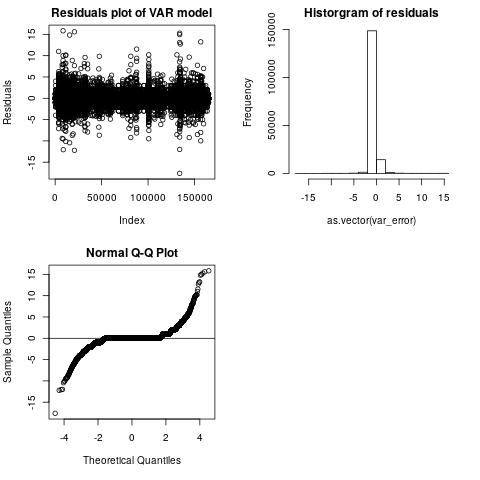
\includegraphics[width=0.8\textwidth, height=0.42\textheight]{Images/Full_VAR_diff_resids.jpg}
    \caption{Residuals for VAR Model}
    \label{fig:Residuals for VAR Model}
\end{figure}

\begin{figure}[H]
    \centering
    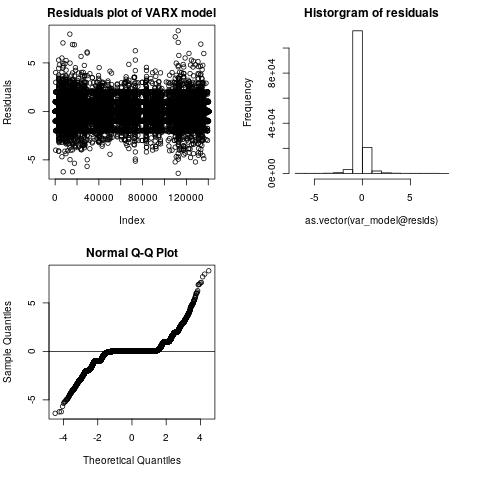
\includegraphics[width=0.8\textwidth, height=0.42\textheight]{Images/Full_VARX_diff_resids.jpg}
    \caption{Residuals for VARX Model}
    \label{fig:Residuals for VARX Model}
\end{figure}

From Figure 11 and 12, we can see that the residuals are mostly randomly scattered and they roughly follow a normal distribution, although it performs rather badly on the lower end and higher end of the outliers. 


\subsubsection{Residuals against Fitted Values}

\begin{figure}[H]
    \centering
    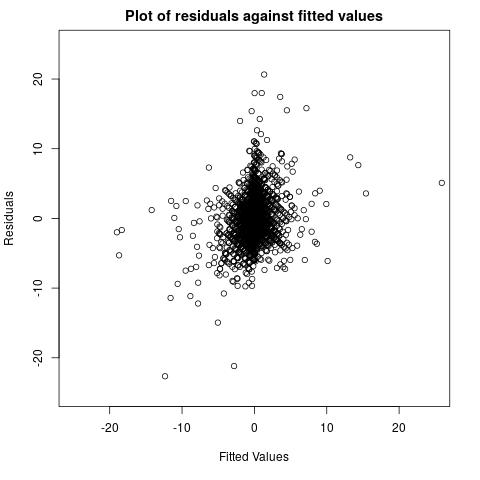
\includegraphics[width=0.6\textwidth, height=0.3\textheight]{Images/Full_VAR_diff_resids_vs_values.jpg}
    \caption{Residuals against Fitted Values for VAR Model}
    \label{fig:Residuals against Fitted Values for VAR Model}
\end{figure}

\begin{figure}[H]
    \centering
    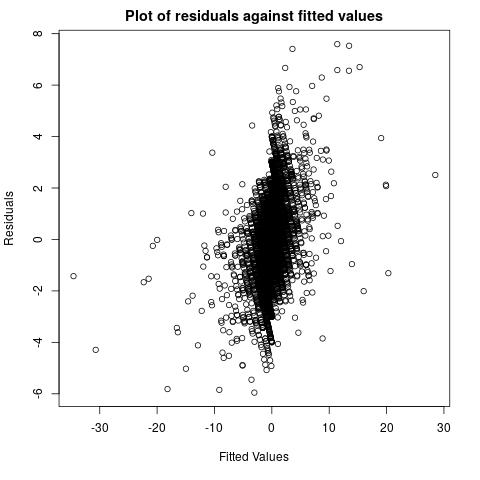
\includegraphics[width=0.6\textwidth, height=0.3\textheight]{Images/Full_VARX_diff_resids_vs_values.jpg}
    \caption{Residuals against Fitted Values for VARX Model}
    \label{fig:Residuals against Fitted Values for VARX Model}
\end{figure}

Figure 13 and 14 shows that heteroscadasticity occurs at the lower and higher ends of the predicted values, whereas in the middle range, the residuals tend to be roughly randomly scattered.

\subsection{Results}
BigVAR library in R was used to implement the VAR models. The MSFE for the VAR model is 76.72 and MSFE for VARX model is 75.63. This would imply that the exogenous variables used do have a moderate amount of explanatory power. 

\section{3-step Approach}

We could then explore an alternative 3-step approach. We would first cluster the locations, then use VAR/VARX to predict the total demand of each cluster, and then assign the total demand to each individual locations. Similar methods can be found in \cite{Paul2015} and \cite{Chi2014}

\subsection{Clustering of locations}

A simple K-means clustering was first done on the locations using their time series data in the training set.

\begin{figure}[H]
    \centering
    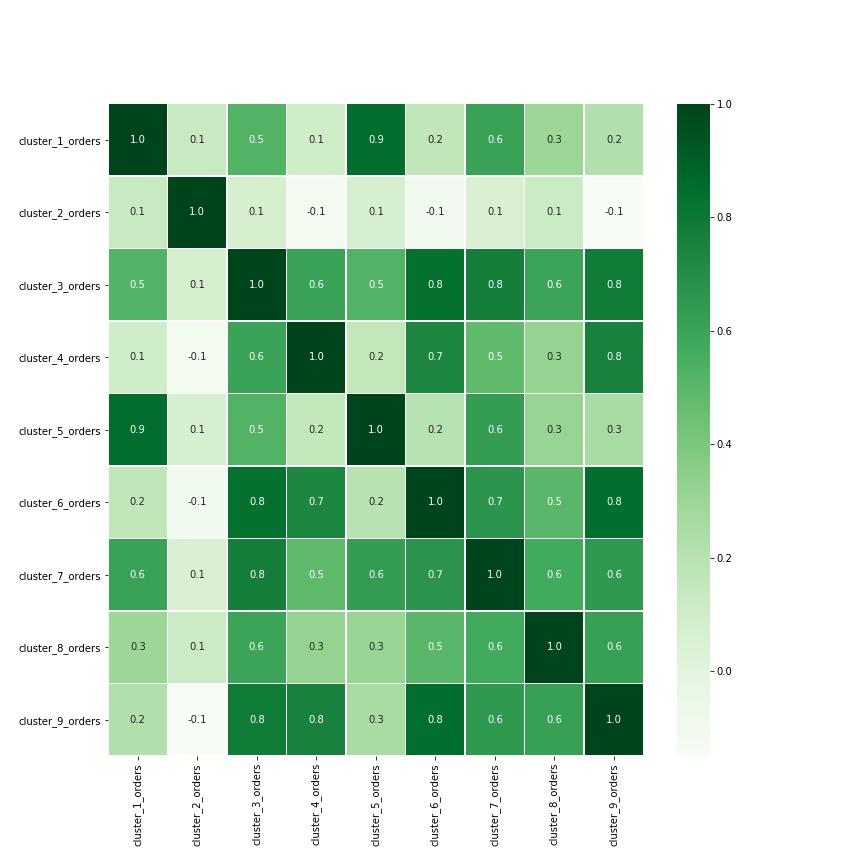
\includegraphics[width=\textwidth, height=0.8\textheight]{Images/cluster_corr_heatmap.jpg}
    \caption{Correlation heatmap for 9 clusters}
    \label{fig:Correlation heatmap for 9 clusters}
\end{figure}

We can see that there exists storng correlation between certain cluster (like cluster 1,5 and cluster 6,9). 

3 different kind of distance metrics are explored to perform K-means clustering. 

\subsubsection{Using longitude/latitude as the distance metric}

Firstly, we would cluster the locations using their geographical longitude and latitude. K-means clustering is performed using the euclidean distance of the locations as the distance metric.  

\subsubsection{Using correlation as the distance metric}

We then also explored using correlation between the time series as the distance metric for K-means clustering. 

\subsubsection{Using Dynamic Time Warping as the distance metric}

Finally, we used Dynamic Time Warping (DTW) Distance as the distance metric for K-means clustering. 

\noindent DTW is one of the commonly-used algorithm for measuring similarity between time series. 
More details on DTW can be found in \cite{Pavel2008}  

\subsection{Predicting total demand for each cluster}

For each type of clustering, a VAR model was then trained on the clusters and the model was used to predict the total demand for each of the clusters. 

\subsection{Assigning total cluster demand to individual locations}

The predicted demand for each cluster would then be reallocated to each individual location in the cluster by:

\begin{center}
    $\displaystyle y_{i} = D_{C(i)} * \frac{(\sum_{j=1}^{n}x_{ij})}{\sum_{l\epsilon C(i)}\sum_{j=1}^{n}x_{lj}}$
\end{center}

\noindent where $y_i$ represents the predicted demand for location i, C(i) represents the cluster which location i belongs to, $D_C(i)$ represents the total demand (from training set) of the cluster C(i), $x_ij$ represents the training set demand at location i at time j

\subsection{Results}

We also test the effect of different number of cluster groups on the MSFE on our full dataset. 

\begin{table}[H]
\begin{tabular}{|l|l|l|l|l|}
\hline
                                                                                                                          & \textbf{3 Clusters} & \textbf{6 Clusters} & \textbf{9 Clusters} & \textbf{12 Clusters} \\ \hline
\textbf{\begin{tabular}[c]{@{}l@{}}Clustering using euclidean\\ distance of latitude/longitude\end{tabular}}              & 61.18               & \textbf{60.67}      & 61.03               & 62.24                \\ \hline
\textbf{\begin{tabular}[c]{@{}l@{}}Clustering using correlation \\ between time series as distance\\ metric\end{tabular}} & 62.22               & \textbf{59.41}               & 61.49               & 61.35       \\ \hline
\textbf{\begin{tabular}[c]{@{}l@{}}Clustering using DTW as\\ distance metric\end{tabular}}                                & 64.00               & 64.37      & 62.68 & \textbf{62.20}                \\ \hline
\end{tabular}
\end{table}

\section{Results and Conclusion}
The table below summarises the results of our models. 

\begin{table}[H]
\begin{tabular}{|l|l|l|ll}
\cline{1-3}
                                                                                                             & \textbf{\begin{tabular}[c]{@{}l@{}}MSFE (Locations with at \\ least 50 non-zero counts)\end{tabular}} & \textbf{MSFE (All locations)} &  &  \\ \cline{1-3}
\textbf{ARIMA}                                                                                               & 47.60                                                                                              & 72.48                         &  &  \\ \cline{1-3}
\textbf{GLM}                                                                                                 & 38.16                                                                                              & 82.42                         &  &  \\ \cline{1-3}
\textbf{VAR}                                                                                                 & 42.76                                                                                              & 76.72                         &  &  \\ \cline{1-3}
\textbf{VARX}                                                                                                & 41.73                                                                                              & 75.63                         &  &  \\ \cline{1-3}
\textbf{\begin{tabular}[c]{@{}l@{}}3-step approach (Using K-means \\ on geographical location)\end{tabular}} & 40.43 & 60.67                        &  &  \\ \cline{1-3}
\textbf{\begin{tabular}[c]{@{}l@{}}3-step approach (Using \\ K-means on correlation \\ of time series)\end{tabular}}           & 39.49 & \textbf{59.41}                         &  &  \\ \cline{1-3}
\textbf{\begin{tabular}[c]{@{}l@{}}3-step approach (Using \\ K-means on DTW \\ of time series)\end{tabular}}           & 40.10 & 62.20                         &  &  \\ \cline{1-3}
\end{tabular}
\end{table}


\noindent We can see that the VAR and VARX model performs better than the GLM models on the full dataset, suggesting that the spatial relationship between locations are useful in forecasting. Also, VARX performs better than VAR model in both cases, suggesting the exogenous variables have some explanatory power and do improve the forecast accuracy. 

\noindent Applying the 3-step forecast also gives a much improved result. This might be due to using a more reliable and reasonable model to predict total demands for just 9 clusters and then re-assigning it to individual locations, rather than having a model to predict all 839 locations, which would intuitively have higher error rate. The method of using VAR on all locations produced a relatively worse result, which is similar to the findings from \cite{Abolfazl2017}, which states that a simple VAR model would not perform as well for high-dimensional data,  

\section{Limitations and Future Work}
Our 3-step approach model display decent MSFE result. Future work could include using neural network, such as Long Short-Term Memory (LSTM) models or Convolutional LSTM models to use spatial-temporal features to forecast the demand across locations.

\section{Appendix}
\subsection{Distribution Plots of Exogenous Variables}
\begin{figure}[H]
    \centering
    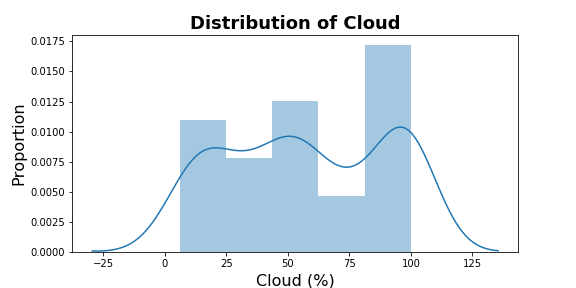
\includegraphics[width=0.6\textwidth, height=0.3\textheight]{Images/distplot_cloud.png}
    \caption{Distribution of Cloud}
    \label{fig:Distribution of Cloud}
\end{figure}

\begin{figure}[H]
    \centering
    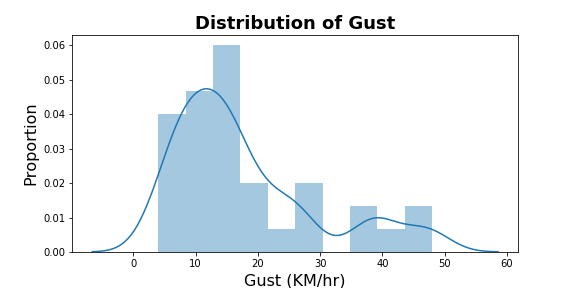
\includegraphics[width=0.6\textwidth, height=0.3\textheight]{Images/distplot_gust.png}
    \caption{Distribution of Gust}
    \label{fig:Distribution of Gust}
\end{figure}

\begin{figure}[H]
    \centering
    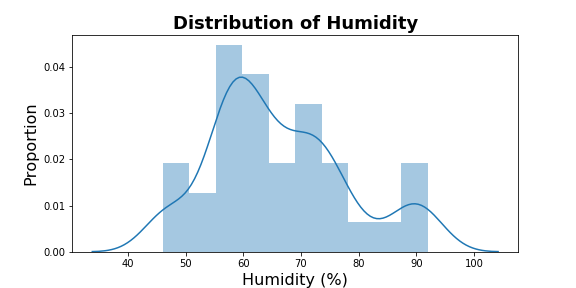
\includegraphics[width=0.6\textwidth, height=0.3\textheight]{Images/distplot_humidity.png}
    \caption{Distribution of Humidity}
    \label{fig:Distribution of Humidity}
\end{figure}

\begin{figure}[H]
    \centering
    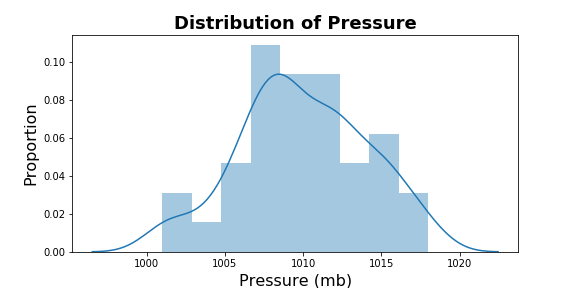
\includegraphics[width=0.6\textwidth, height=0.3\textheight]{Images/distplot_pressure.png}
    \caption{Distribution of Pressure}
    \label{fig:Distribution of Pressure}
\end{figure}

\begin{figure}[H]
    \centering
    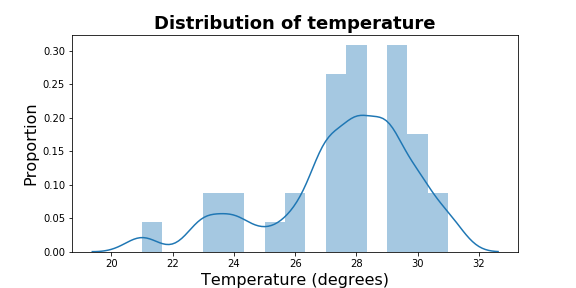
\includegraphics[width=0.6\textwidth, height=0.3\textheight]{Images/distplot_temp.png}
    \caption{Distribution of Temperature}
    \label{fig:Distribution of Temperature}
\end{figure}

\begin{figure}[H]
    \centering
    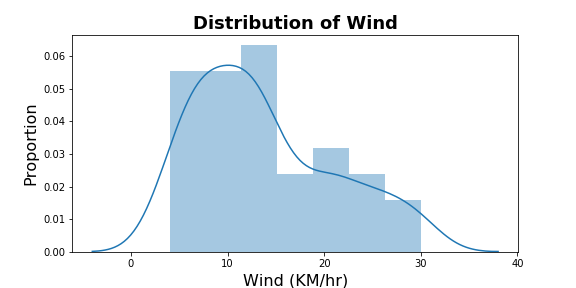
\includegraphics[width=0.6\textwidth, height=0.3\textheight]{Images/distplot_wind.png}
    \caption{Distribution of Wind}
    \label{fig:Distribution of Wind}
\end{figure}

\subsection{Mean Demand Against Exogenous Variables}

\begin{figure}[H]
    \centering
    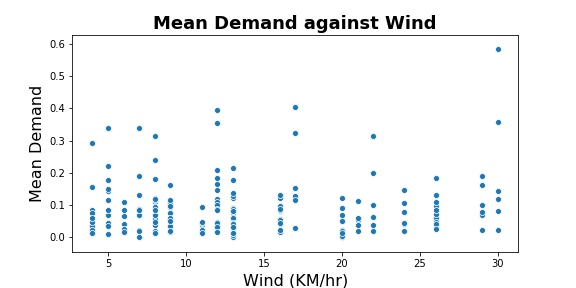
\includegraphics[width=0.6\textwidth, height=0.3\textheight]{Images/wind_mean_demand.jpg}
    \caption{Mean Demand against Wind}
    \label{fig:Mean Demand against Wind}
\end{figure}

\begin{figure}[H]
    \centering
    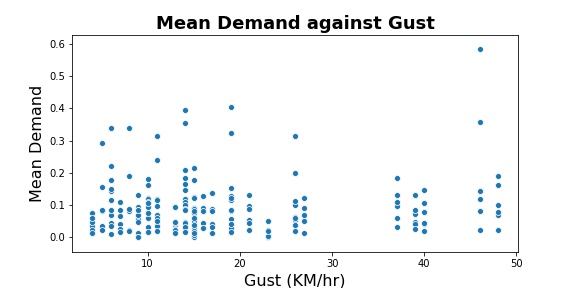
\includegraphics[width=0.6\textwidth, height=0.3\textheight]{Images/gust_mean_demand.jpg}
    \caption{Mean Demand against Gust}
    \label{fig:Mean Demand against Gust}
\end{figure}

\begin{figure}[H]
    \centering
    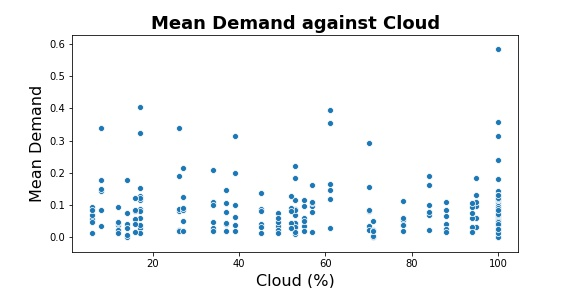
\includegraphics[width=0.6\textwidth, height=0.3\textheight]{Images/cloud_mean_demand.jpg}
    \caption{Mean Demand against Cloud}
    \label{fig:Mean Demand against Cloud}
\end{figure}

\begin{figure}[H]
    \centering
    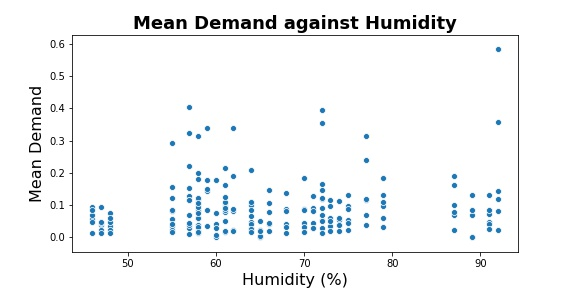
\includegraphics[width=0.6\textwidth, height=0.3\textheight]{Images/humidity_mean_demand.jpg}
    \caption{Mean Demand against Humidity}
    \label{fig:Mean Demand against Humidity}
\end{figure}

\begin{figure}[H]
    \centering
    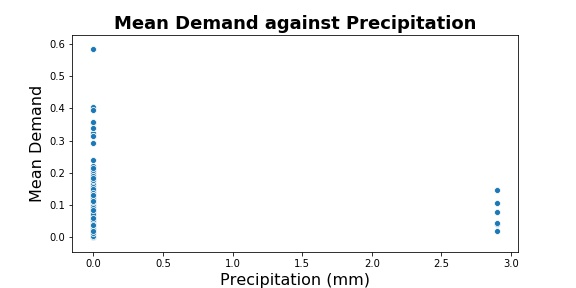
\includegraphics[width=0.6\textwidth, height=0.3\textheight]{Images/prec_mean_demand.jpg}
    \caption{Mean Demand against Precipitation}
    \label{fig:Mean Demand against Precipitation}
\end{figure}

%%%%%%%%%%%%%%%%%%%%%%%%%%%%%%%%%%%%%%%%%%%%%%%%%%%%%%%%%%%%
%%% Bibliography
%%%%%%%%%%%%%%%%%%%%%%%%%%%%%%%%%%%%%%%%%%%%%%%%%%%%%%%%%%%%
\bibliographystyle{apa} 
\bibliography{references}


\end{document}
